% if you want to include some content outside of frames also in slides, use \mode<
\mode<beamer|article>{
  \title{Structured Presentation Template}
  \author{Michal Hoftich}
  \maketitle
}

\tableofcontents

\section{Introduction}


This template is designed for presentations that need more than just slides.
It lets you create both the talk itself and a more detailed handout with notes and
commentary. That way, you can generate everything from a single source—both the
material for the live talk and something useful for people who didn’t attend.

It includes several main source files, each with a specific purpose:

\begin{frame}[fragile]{Overview of Files}
  \begin{itemize}
   \item \textbf{\texttt{slides.tex}} 
   \item \textbf{\texttt{handout.tex}}
   \item \textbf{\texttt{presentation.tex}}
   \item \textbf{\texttt{preamble.tex}}
   \item \textbf{\texttt{config.cfg}}
  \end{itemize}
\end{frame}
\begin{itemize}
  \item \textbf{\texttt{slides.tex}} – This file is used to generate the main
    presentation in Beamer format. It contains the content that is shown during
    the talk.
  
  \item \textbf{\texttt{handout.tex}} – A handout version of the presentation,
    formatted as a standard article. In addition to the visible content from
    the slides, it includes supplementary notes and commentary that do not
    appear in the presentation itself. This file is intended to be distributed
    after the presentation and should be self-contained, so that it is useful
    even to those who did not attend the talk.
  
  \item \textbf{\texttt{presentation.tex}} – This file contains the full source
    text of the presentation. Content written inside
    \verb|\begin|\verb|{frame}...\end{frame}| blocks is included both in the
    \texttt{slides.tex} and \texttt{handout.tex} outputs. Any text outside of
    frames is excluded from the presentation but included in the handout. This
    allows the author to provide detailed commentary, background, or additional
    explanation that supports the talk.

  \item \textbf{preamble.tex} – This file includes packages or defines commands
    used in the presentation.

  \item \textbf{config.cfg} – This file contains configuration options for
    \TeX4ht. For example CSS styles used in the web version of this document,
    or redefinitions of \LaTeX\ commands.

\end{itemize}

You can edit these files to customize the presentation and handout to your
needs. At the minimum, you will want to replace contents of
\texttt{presentation.tex} with your own text, and you may also want to modify
the \texttt{preamble.tex} file to include any additional packages or commands
you need.

\section{Basic Usage}

\begin{frame}[fragile]{Create a New Github Repository}
  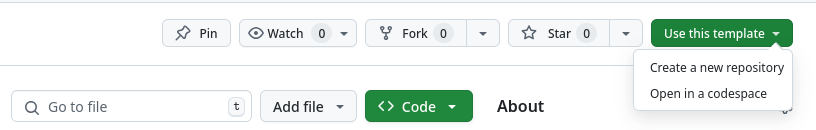
\includegraphics[width=\textwidth]{img/template-use.png}
\end{frame}

To start your own presentation using this template, click the "Use this
template" button at the top of the GitHub repository page. This will create a
new repository in your account with the same structure and files. You can then
clone it, customize the content, and start building your own slides and
handouts.


\begin{frame}[fragile]{Usage of Frames and Handout Commentary}

  \begin{block}{}
    A basic syntax of the document used in \verb|presentation.tex| is following:
  \end{block}

\begin{likeverbatim}  
  \verb|\begin{frame}{Frame title}|\\
  \verb|contents of the frame...|\\
  \verb|\end|\verb|{frame}|\\
  \vspace{1em}
  \verb|Commentary included in the handout|
\end{likeverbatim}

\end{frame}

For example, source code of one of the previous frames looks like this:

\verb|\begin|\verb|{frame}[fragile]{Overview of Files}|
\begin{verbatim}
  \begin{itemize}
   \item \textbf{\texttt{slides.tex}} 
   \item \textbf{\texttt{handout.tex}}
   \item \textbf{\texttt{presentation.tex}}
   \item \textbf{\texttt{preamble.tex}}
  \end{itemize}
\end{verbatim}
\verb|\end|\verb|{frame}|
\begin{verbatim}
\begin{itemize}
  \item \textbf{\texttt{slides.tex}} – This file is used to generate the main 
  presentation in Beamer format. It contains the content that is shown during the talk.
\end{verbatim}

The content inside the \verb|\begin|\verb|{frame}...\end|\verb|{frame}| block is included in both
the presentation and the handout, but the \texttt{itemize} environment that follows
the \verb|frame| environment is only included in the handout.


\begin{frame}[fragile]{Shared Content Outside of Frames}

\begin{verbatim}
\mode<beamer|article>{
  \title{Structured Presentation Template}
  \author{Michal Hoftich}
  \maketitle
}
  
\end{verbatim}
\end{frame}

You can use the \verb+\mode<beamer|article>{...}+ command to include content that should be
shown in both the presentation and the handout. This can be useful for
the presentation title or table of contents, for example.




\section{Compiling the Presentation}

\begin{frame}[fragile]{How to Compile to PDF} 

To compile the presentation or the handout to PDF using LuaLaTeX, run the following commands:

\begin{verbatim}
$ lualatex slides.tex
$ lualatex handout.tex
\end{verbatim}
\end{frame}

You can compile the output files using any standard \LaTeX\ distribution that includes Beamer and the necessary packages.

\begin{frame}[fragile]{HTML Version}
  Use \href{https://www.tug.org/tex4ht/}{\TeX4ht} to compile the presentation to HTML format. 
\begin{verbatim}
$ make4ht -c config -l handout.tex    
\end{verbatim}

The \verb|-l| option  ensures that Lua\LaTeX\ is used as the compiler. 
\end{frame}


The HTML version is built from the article-style handout, not the Beamer slides.
This makes it better suited for the web or long-term sharing, since it includes
all explanations and doesn’t depend on slide layout.

\begin{frame}[fragile]{\TeX4ht Configuration}

\begin{block}{}
CSS declaration for the table of contents links color:
\end{block}
  
\begin{verbatim}
\Css{.tableofcontents a {color: \#0f0f0f;}}
\Css{.tableofcontents a:hover {color: \#6f5f4f;}}
\end{verbatim}
\end{frame}

You can customize the appearance of the output by editing the \texttt{config.cfg} file.
The above example shows how to change the color of links in the table of contents.
You may also want to change the background color of the TOC. Note that 
if you want to use CSS RGB colors, you need to use the \verb|\#| character.

You can find more information about \TeX4ht configuration files in the 
\href{https://www.kodymirus.cz/tex4ht-doc/Configurations.html}{\TeX4ht documentation}.


\section{Automated HTML Output}

This section explains how \href{https://docs.github.com/en/actions/writing-workflows/quickstart}{GitHub Actions}
is used to automatically generate and publish an HTML version of the handout whenever changes are pushed to the \texttt{main} branch.

The output is built using \texttt{make4ht} and published to the \texttt{gh-pages} branch,
making it easy to share a web-readable version of the talk.

\begin{frame}[fragile]{GitHub Actions Overview}
Key parts of the workflow that builds and publishes the HTML:

\begin{verbatim}
- name: Run make4ht
  uses: xu-cheng/texlive-action/full@v1
  with:
    run: |
      make4ht -lj index -a debug -d out handout.tex

- name: Publish the web pages
  uses: peaceiris/actions-gh-pages@v3
  with:
    github_token: ${{ secrets.GITHUB_TOKEN }}
    publish_dir: ./out
\end{verbatim}

\end{frame}


The workflow is defined in \texttt{.github/workflows/main.yml}.
You can edit this file to customize the build process, such as changing the options passed to \texttt{make4ht}.

It uses two GitHub Actions: \href{https://github.com/xu-cheng/texlive-action}{xu-cheng/texlive-action}
and \href{https://github.com/peaceiris/actions-gh-pages}{peaceiris/actions-gh-pages}.
The first one lets you use any command available in the TeX Live installation, such as \texttt{make4ht} or \texttt{lualatex}.
The second one publishes the contents of a specified directory to the \texttt{gh-pages} branch of your repository,
which is used by GitHub Pages to serve static content.



\begin{frame}[fragile]{Automatic HTML Build}
Changes pushed to \texttt{main} branch trigger a GitHub Actions workflow that:

\begin{itemize}
  \item Compiles \texttt{handout.tex} to HTML using \texttt{make4ht}
  \item Publishes the output to the \texttt{gh-pages} branch
\end{itemize}

The command used is:

\begin{verbatim}
make4ht -lj index -a debug -d out handout.tex
\end{verbatim}
\end{frame}


This builds the HTML into the \texttt{out/} folder, which is then published
using the \texttt{peaceiris/actions-gh-pages} action, specified by the
\texttt{publish\_dir} setting.


\begin{frame}[fragile]{Why \texttt{-j index}?}
\begin{itemize}
  \item The \texttt{-lj index} option is a shorthand for \texttt{-l -j index}
  \item The \texttt{-j index} option sets the HTML output filename to \texttt{index.html}
  \item This lets you use clean URLs like:
  
\begin{verbatim}
https://username.github.io/repo/
\end{verbatim}

\end{itemize}
\end{frame}


There’s no need to specify the filename in the link — GitHub Pages
automatically looks for \texttt{index.html} by default. This makes it easier to share
the presentation and helps avoid broken links due to filename mismatches.

For example, this presentation is available at: \url{https://michal-h21.github.io/tex4ht-presentation/}.

\section{Github Pages}

\begin{frame}[fragile]{Github Actions Interface}
  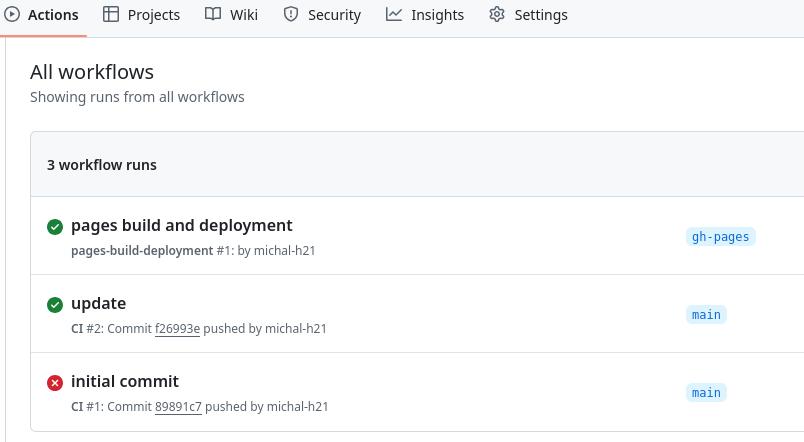
\includegraphics[width=\textwidth]{img/github-actions.png}
\end{frame}

After you push changes to the \texttt{main} branch, you can check the \texttt{Actions} tab in your
Github repository. It shows the status of the workflow, including whether it ran successfully or if there were any errors.


\begin{frame}[fragile]{Errors}
  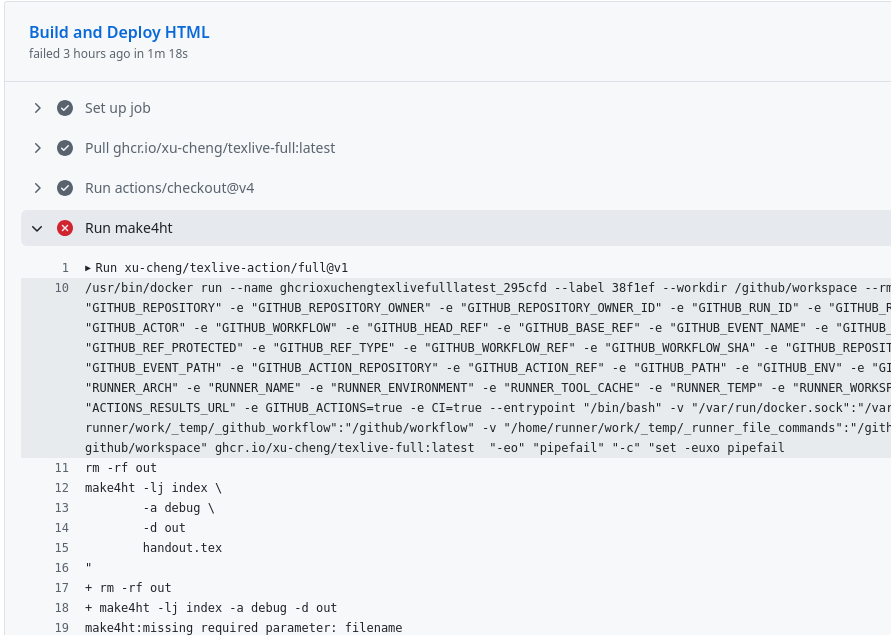
\includegraphics[width=\textwidth]{img/github-error.png}
\end{frame}


You can also check the logs of the workflow run to see what went wrong.
If you encounter an error, it will be displayed in the logs, and you can use that
information to debug the issue.

In this case, the filename of the TeX file was incorrect. I had to fix the filename in the GitHub Actions YAML file.


\begin{frame}[fragile]{Setup Github Pages}
  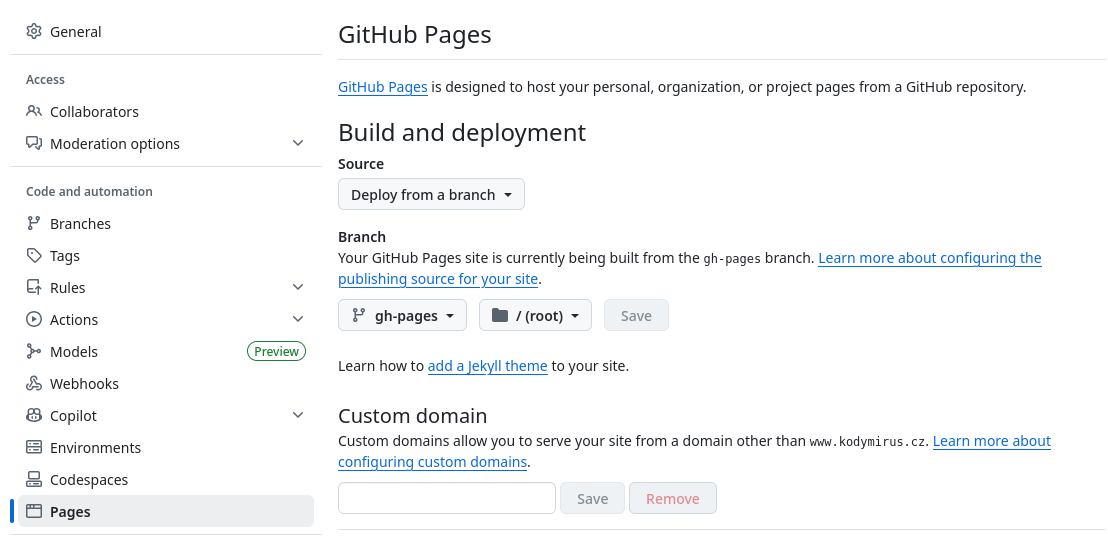
\includegraphics[width=\textwidth]{img/github-pages.png}
\end{frame}

Once the workflow runs successfully, you can set up GitHub Pages to serve the \texttt{gh-pages} branch.

All output files produced by \texttt{make4ht} will be served on the web.
They will be available at:
\verb|https://username.github.io/repo/|,
where \texttt{username} is your GitHub username and \texttt{repo} is the name of your repository.

